\documentclass{article}
\title{Sistema de controle de mesa de som - Sistemas digitais e microcontrolados}
\date{}

\usepackage[utf8]{inputenc}
\usepackage[portuguese]{babel}
\usepackage[margin=2.5cm,headheight=0pt,headsep=0pt]{geometry}
\usepackage{amsmath}
\usepackage{physics}
\usepackage{titlesec}
\usepackage{graphicx}
\usepackage{wrapfig}
\usepackage{caption}
\usepackage{subcaption}
\usepackage{karnaugh-map}
\usepackage{setspace}
\usepackage[parfill]{parskip}
\usepackage[nottoc]{tocbibind}
\usepackage[backend=biber]{biblatex}
\addbibresource{/home/luispengler/drive/NextCloud/Research/read/bib.bib}
\usepackage{authblk}
\author[1]{Giovanna Bughi}
\author[2]{Gustavo Ratier Cardoso}
\author[3]{João Vitor Medeiros}
\author[4]{Luís Spengler}
\affil[1,2,3,4]{Instituto Federal de Educação, Ciência e Tecnologia de Mato Grosso do Sul}

\graphicspath{{./docs/}}

\renewcommand{\baselinestretch}{1.5}

\doublespacing

\begin{document}
\maketitle

\tableofcontents

\medskip

\vspace{500mm}
\section{Problema proposto}
Para a mesa de som são conectados três microfones em uma única caixa de som amplificada, que são: ChP, ChD e ChC. A sigla “Ch” vem da palavra derivada do inglês, Channel (Canal), já as letras que à acompanham são do Presidente, Diretor e Coordenador, respectivamente. Foi identificado o nível de prioridade entre os microfones conforme sua transmissão e elaborado o circuito lógico combinacional que permitirá ligar os microfones segundo sua ordem de prioridade conforme a relação abaixo:

Prioridade 1: Presidente;

Prioridade 2: Diretor;

Prioridade 3: Coordenador.

Seu acionamento é simples, cada microfone é acionado pelo usuário através de um interruptor (liga-desliga) que nesse caso, serão também as entradas. Os microfones quando acionados comutam em sua saída 0 ou 1, informando ao circuito lógico que, por sua vez, aciona uma das saídas (SP, SD, SC) na caixa amplificada. Então, quando o Presidente ligar seu microfone, terá prioridade sobre os demais. Quando o Diretor ligar seu microfone, só terá prioridade sobre o Coordenador. E por fim, o Coordenador só falará quando os demais microfones não estiverem ligados.

\vspace{15mm}
\begin{center}
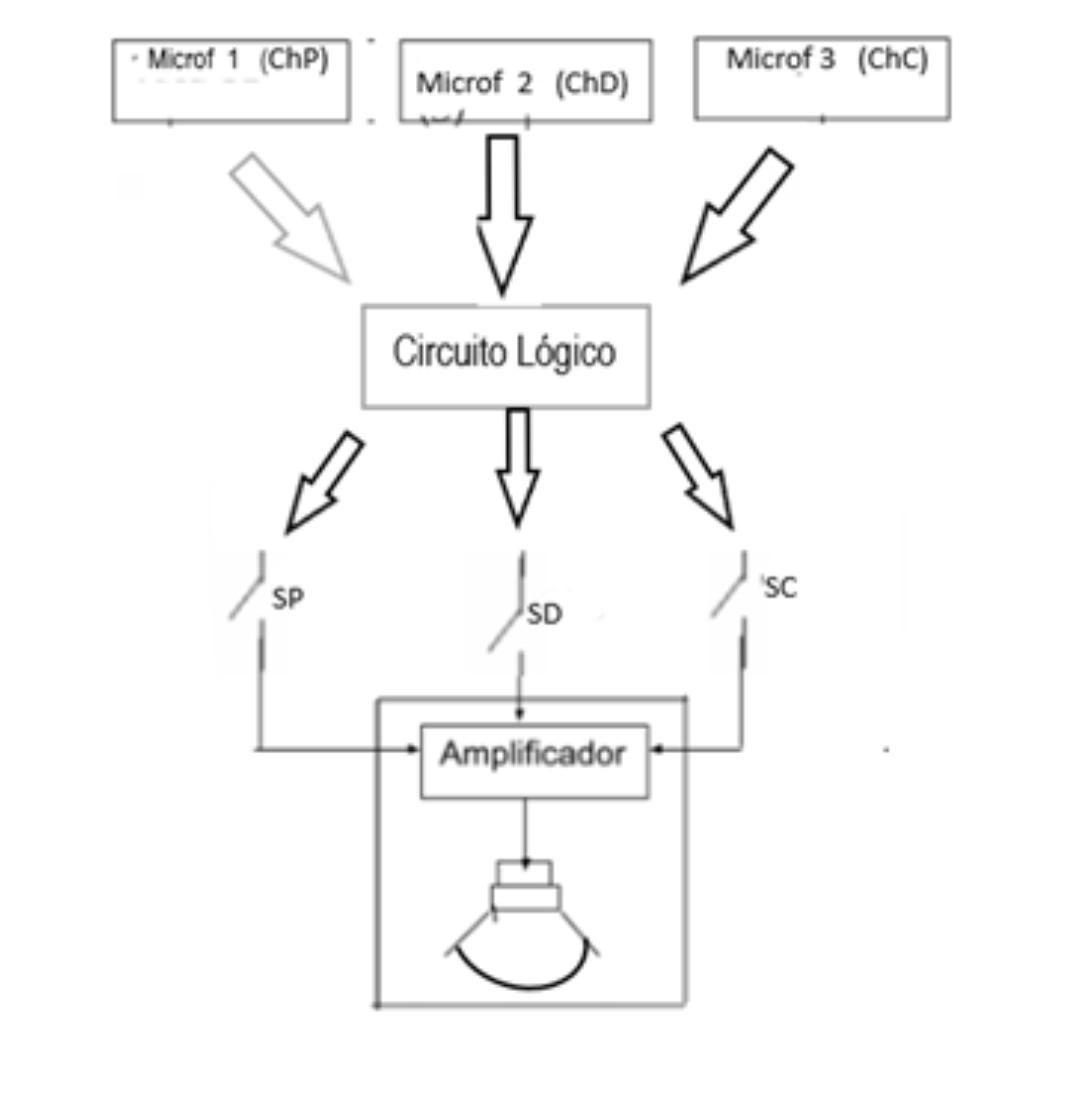
\includegraphics[width=0.5\textwidth]{esbocoroubado}
\end{center}

\section{Solução do problema proposto}

\subsection{Identificação das variáveis de entrada e saída}
Identificado o problema proposto, foram denominadas as entradas e saídas que serão utilizadas para a ativação dos microfones no circuito lógico. A sigla “Ch” é originada do inglês Channel, em que canal é a sua tradução; a entrada será referente ao canal de seus utilizadores conforme sua prioridade; a letra S nas expressões lógicas é representada por saída e será utilizada para denominar a saída do utilizador. Então ChP; ChD; ChC; SP; SD e SC serão os canais de entrada e expressão de saída do Presidente, Diretor e Coordenador respectivamente, de acordo com suas siglas e letras.

\subsection{Identificação dos estados das variáveis de entrada e saída}
Nas entradas ChP, ChD e ChC terão nível lógico alto (1), somente quando os usuários tiverem seus microfones ligados; se todos tiverem seus microfones ligados: ChP = 1, ChD = 1 e ChC = 1; em estado inicial todas as inicias serão iguais a zero (0), então: ChP = 0, ChD = 0, ChC = 0. Conforme a conversa prossegue e os usuários ativam o microfone, são alteradas as variáveis de saída para estado lógico alto (1).

\subsection{Montagem da tabela verdade}
Reunidas as variáveis de entrada e saída, uma tabela verdade foi feita a fim de determinar os estados de atuação em cada uma das entradas e saídas, obedecendo a ordem de prioridade em cada falante de acordo com os valores da tabela abaixo:

\begin{displaymath}
\begin{array}{|c c c|c c c|}
INPUT & & & OUTPUT &\\
\hline
ChP & ChD & ChC & SP & SD & SC\\
\hline % Put a horizontal line between the table header and the rest.
0 & 0 & 0 & 0 & 0 & 0\\
0 & 0 & 1 & 0 & 0 & 1\\
0 & 1 & 0 & 0 & 1 & 0\\
0 & 1 & 1 & 0 & 1 & 0\\
1 & 0 & 0 & 1 & 0 & 0\\
1 & 0 & 1 & 1 & 0 & 0\\
1 & 1 & 0 & 1 & 0 & 0\\
1 & 1 & 1 & 1 & 0 & 0\\
\end{array}
\end{displaymath}

\subsection{Obtenção da expressão de saída}
A partir da tabela verdade, foram equacionadas as expressões de saída referente ao seu proprietário.

\begin{enumerate}
	\item SP (Saída do Presidente) em Função de ChP (Canal do Presidente);
		\[SP=ChP\cdot ChC' + ChP\cdot ChC\]
		\[SP=ChP\cdot (ChC' + ChC)\]
		\[SP=ChP\]
	\item SD (Saída do Diretor) em Função de ChD (Canal do Diretor);
		\[SD=ChP'\cdot ChD\]
	\item SC (Saída do Coordenador) em Função de ChC (Canal do Coordenador).
		\[SC=(ChP'\cdot ChD')\cdot ChC\]
\end{enumerate}

\subsection{Mapa de Karnaugh}
Mapa de Karnaugh para a saída do presidente (SP)

\begin{karnaugh-map}*[4][2][1][$ChPChD$][$ChC$]
	\minterms{2,3,6,7}
	\maxterms{0,1,4,5}
	\indeterminants{2,5}
	\implicant{3}{2}
	\implicant{7}{6}
\end{karnaugh-map}

Mapa de Karnaugh para a saída do diretor (SD)

\begin{karnaugh-map}*[4][2][1][$ChPChD$][$ChC$]
	\maxterms{0,2,3,4,6,7}
	\minterms{1,5}
	\implicant{1}{5}
\end{karnaugh-map}

Mapa de Karnaugh para a saída do coordenador (SC)

\begin{karnaugh-map}*[4][2][1][$ChPChD$][$ChC$]
	\maxterms{0,1,2,3,5,6,7}
	\minterms{4}
	\implicant{4}{4}
\end{karnaugh-map}

\subsection{Simplificação da expressão através do mapa de Karnaugh}
Analisando o mapa de Karnaugh é possível identificar que, apenas a expressão referente ao Presidente (SP em função de ChP) será simplificada por ser a única com alguma propriedade de simplificação.

\begin{karnaugh-map}*[4][2][1][$ChPChD$][$ChC$]
	\minterms{2,3,6,7}
	\maxterms{0,1,4,5}
	\indeterminants{2,5}
	\implicant{3}{2}
	\implicant{7}{6}
\end{karnaugh-map}

\subsection{Circuito lógico}

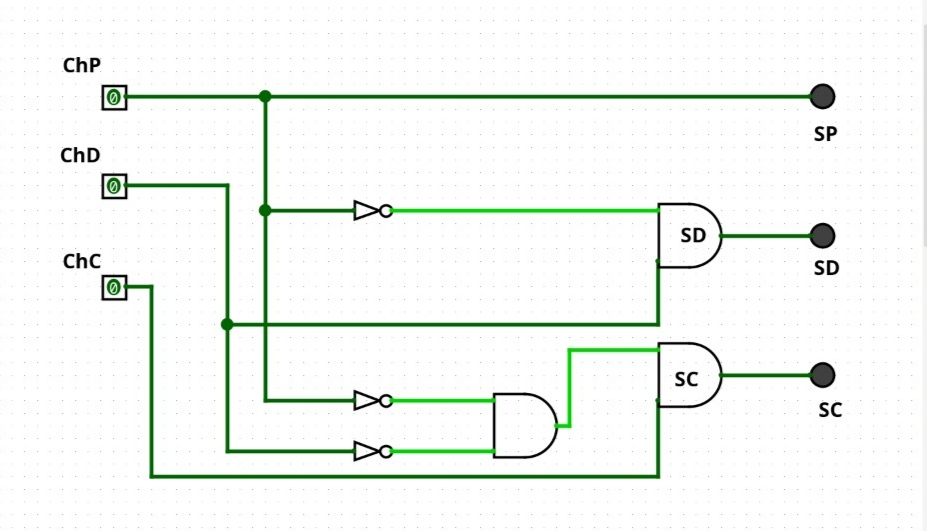
\includegraphics[width=\textwidth]{circuito}

\subsection{Componentes utilizados no circuito}
\begin{enumerate}
	\item Board de instrumentação e controle possuindo suporte para as protoboards;
	\item CI (AND) SN7408N e CI (NOT) SN7404N;
	\item Jumper de ligação (macho-macho) e Jumper de ligação (macho-fêmea);
	\item Fios de conexão para alimentação do circuito ligados no GND de cada CI; 
	\item Fios de conexão para alimentação do circuito ligados no VCC de cada CI.
	\item Chaves de acionamento para cada lógica no circuito.
\end{enumerate}

\section{Conclusão}
Com o circuito montado, programado e funcionando conforme os parâmetros apresentados, ao acionar as chaves, cada uma delas são executadas conforme o grau de prioridade no alto falante determinado pelos Cis. O Presidente ao solicitar a transmissão no alto falante o somente seu canal será reproduzido e impossibilitando os demais serem de serem reproduzidos; ao Diretor solicitar reprodução do seu microfone no alto falante, somente ele fará. A menos que o Presidente reproduza seu microfone uma outra vez; e o Coordenador só falará quando os microfones do Presidente e do Diretor não forem reproduzidos, respectivamente. Através dessas relações, se vê na prática a aplicação da ordem de prioridade conforme demonstrada no tópico “Problema Proposto”. O circuito e seu funcionamento são um sucesso e atuam conforme o solicitado.

\medskip

\end{document}
